%%%%%%%%%%%%%%%%%%%%%%%%%%
% NUMERICAL CASE STUDIES %
%%%%%%%%%%%%%%%%%%%%%%%%%%
In order to illustrate the power and versatility of the devised framework we conduct a selection of computer experiments.
This shall be seen as a proof of concept and benchmark of the proposed methodology in the context of engineering applications.
% FORWARD PROBLEM: MULTIPLE BEAMS
A system of identically designed structural components functions as the basis for probing a range of experimental scenarios.
Specifically we deal with an ensemble of simply supported beams that are tested in a series of three-point bending experiments.
% INVERSE PROBLEMS UNDER UNCERTAINTY
By multilevel analysis of measured beam deflections we highlight how different inferential goals, e.g.\ probabilistic inversion, residual calibration or optimal combination of information,
can be achieved in the presence of material variability and uncertainties in the experimental setup.
% DETERMINISTIC MODELING
Keeping deterministic modeling simple and intuitive will allow us to focus on uncertainty quantification aspects that are the essential subject matter of this research.
% COMPUTATIONAL OBSTACLES
Incidentally we learn about the computational obstacles that must be overcome when aiming at ``real-world'' applications.
\par % SECTION OUTLINE
The forward problem will be shortly introduced in \cref{sec:PEM:CaseStudies:Beams}.
Around this submodel, that covers the deterministic features of the system, Bayesian multilevel models will be built to capture uncertainty and variability.
Probabilistic inversion, i.e.\ deducing the material variability throughout an ensemble of similar specimens, will be tackled in \cref{sec:PEM:CaseStudies:ProbInv}.
The subsequent \cref{sec:PEM:CaseStudies:ResCal} will deal with residual model calibration.
In \cref{sec:PEM:CaseStudies:AddPres} the impact of prescribed uncertainties in the test conditions will be investigated.
In \cref{sec:PEM:CaseStudies:CombInf} borrowing strength will be utilized in order to ideally estimate the material characteristics of a single specimen by using information obtained from the other specimens.

%%%%%%%%%%%%%%%%%%%%%%%%%%%%%%%%%%%%%%%%%%%%%%%%%%%%%%%%%%%%%%%%%%%%%%%%%%%%%%%%%%%%%%%%%%%%%%%%%%%%%%%%%%%%%%%%%%%%%%%%%%%%%%%%%%%%%%%%%%%%%%%%%%%%%%%%%%%%%%%%%%%%%%%%%%%%%%%%%%%%%%%%%
\subsection{Mechanical model} \label{sec:PEM:CaseStudies:Beams}
%%%%%%%%%%%%%%%%%%%%
% MECHANICAL MODEL %
%%%%%%%%%%%%%%%%%%%%
The system under consideration is an ensemble of identically manufactured beams \(i=1,\ldots,n\) with well-known lengths \(L_i\) and rectangular cross sections with widths \(b_i\) and heights \(h_i\).
Yet the completed beams are only similar in the sense that we assume variability in the elastic moduli \(E_i\) across the ensemble, e.g.\ due to slight irregularities in the fabrication process.
For each single beam \(i\) the Young's modulus \(E_i\) is assumed to be constant along the main beam axis.
% FORWARD FORMULA
The deflections \(\perfect{v}_i(s_{i,j})\) of a simply supported beam \(i\) under a concentrated point load \(F_i\) at midspan can be easily derived in Euler-Bernoulli beam theory.
For positions \(s_{i,j}\) along the beam axis with \(0 \leq s_{i,j} \leq L_i/2\) and \(j=1,\ldots,n_i\) the deflections follow as
\begin{equation} \label{eq:PEM:Beams:AlgebraicFormula}
  \perfect{v}_i(s_{i,j}) = \frac{F_i s_{i,j} }{48 E_i I_i} \left(3 L_i^2 - 4s_{i,j}^2 \right), \;\, \text{for} \;\, 0 \leq s_{i,j} \leq L_i/2,
\end{equation}
where the moment of inertia is given as \(I_i = b_i h_i^3 / 12\).
Likewise a symmetric expression holds for positions \(s_{i,j}\) along the main axis with \(L_i/2 \leq s_{i,j} \leq L_i\).
% SIMPLY SUPPORTED BEAM
A single simply supported beam is visualized in \cref{fig:PEM:Beams:SimpleBeam}.
\begin{figure}[ht]
  \centering
  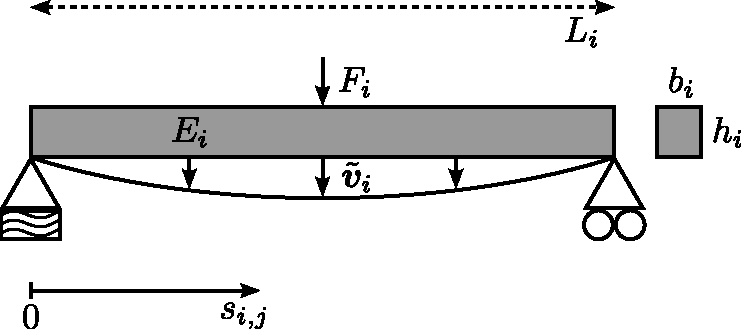
\includegraphics[width=\PEMbeamWidth]{fig_PEM_SimpleBeam}
  \caption[A simply supported beam]{A simply supported beam.}
  \label{fig:PEM:Beams:SimpleBeam}
\end{figure}
\par % VECTORIZATION
Together with its symmetric counterpart, the algebraic formula \cref{eq:PEM:Beams:AlgebraicFormula} constitutes the deterministic submodel of the system under consideration.
When a load \(F_i\) is applied to a beam \(i\) with physical dimensions \(\bm{l}_i = (L_i,b_i,h_i)\) and an elastic modulus \(E_i\),
these relations predict the deflections \(\perfect{\bm{v}}_i = (\perfect{v}_i(s_{i,1}),\ldots,\perfect{v}_i(s_{i,n_i}))\) at positions \(\bm{s}_i = (s_{i,1},\ldots,s_{i,n_i})\).
We denote this as
\begin{equation} \label{eq:PEM:Beams:ForwardModel}
  \perfect{\bm{v}}_i = \mathcal{M}(E_i,F_i,\bm{l}_i,\bm{s}_i).
\end{equation}
% UNCERTAINTY MODELS
When beam deflections are measured in three-point bending tests for each member \(i=1,\ldots,n\) in the population,
multilevel inversion allows for optimal data analysis in experimental situations where the inputs of \cref{eq:PEM:Beams:ForwardModel} are subject to uncertainty.

%%%%%%%%%%%%%%%%%%%%%%%%%%%%%%%%%%%%%%%%%%%%%%%%%%%%%%%%%%%%%%%%%%%%%%%%%%%%%%%%%%%%%%%%%%%%%%%%%%%%%%%%%%%%%%%%%%%%%%%%%%%%%%%%%%%%%%%%%%%%%%%%%%%%%%%%%%%%%%%%%%%%%%%%%%%%%%%%%%%%%%%%%
\subsection{Probabilistic inversion} \label{sec:PEM:CaseStudies:ProbInv}
%%%%%%%%%%%%%%%%%%%%%%%%%%%
% PROBABILISTIC INVERSION %
%%%%%%%%%%%%%%%%%%%%%%%%%%%
We begin with Bayesian probabilistic inversion, on the basis of which we demonstrate how one can quantify the material variability within the ensemble of beams in a series of bending tests.
A numerical experiment is therefore set up as follows.
% EXPERIMENTAL SETUP
We consider a number of \(n=100\) beams with well-known dimensions \(L_i=\unit[1]{m}\) and \(b_i=h_i=\unit[10]{cm}\).
Beams are subjected to concentrated loads \(F_i=\unit[30]{kN}\) that are applied at midspan.
For \(i=1,\ldots,100\) Young's moduli \(E_i\) are independently sampled from a lognormal distribution \(\mathcal{LN}(E_i \cond \mu_E,\sigma_E)\) with mean \(\mu_E=\unit[15]{GPa}\) and standard deviation \(\sigma_E=\unit[3]{GPa}\).
This corresponds to a coefficient of variation \(c_{E} = \unit[20]{\%}\).
% TREATED AS UNKNOWNS
After having set up the experiment, the hyperparameters \(\bm{\theta}_E=(\mu_E,\sigma_E)\) as well as beam-specific moduli \(E_i\) will be treated as unknowns. 
% PREDICTED DEFLECTIONS
At \(n_i=3\) positions \(\bm{s}_i = (s_{i,1},s_{i,2},s_{i,3})\) with \(s_{i,1}=\unit[25]{cm}\), \(s_{i,2}=\unit[50]{cm}\) and \(s_{i,3}=\unit[75]{cm}\)
beam deflections \(\perfect{\bm{v}}_i = (\perfect{v}_i(s_{i,1}),\perfect{v}_i(s_{i,2}),\perfect{v}_i(s_{i,3}))\) are computed according to \cref{eq:PEM:Beams:AlgebraicFormula}.
% MEASUREMENT UNCERTAINTY
In order to take measurement uncertainty and forward model imperfection into account, we perturb the predictions \(\perfect{\bm{v}}_i\) with noise terms \(\bm{\varepsilon}_i = (\varepsilon_{i,1},\varepsilon_{i,2},\varepsilon_{i,3})\).
Those terms are independently sampled from Gaussian distributions \(\mathcal{N}(\bm{\varepsilon}_i \distparam \bm{0},\bm{\Sigma}_i)\) with \(\bm{\Sigma}_i = \sigma_i^2 \bm{I}_3\) and \(\sigma_i = \unit[0.1]{mm}\).
% PSEUDO DATA & INFERENTIAL GOAL
Eventually \(\bm{v}_i = \perfect{\bm{v}}_i + \bm{\varepsilon}_i\) represent the pseudo data that will become analyzed with respect to the QoI \(\bm{\theta}_E = (\mu_E,\sigma_E)\).
\par % HYPERPRIOR MODEL
In many circumstances expert knowledge about the QoI \(\bm{\theta}_E\) is available prior to analyzing the data.
This knowledge can be accounted for by eliciting a suitable prior distribution \(\pi(\bm{\theta}_E)\).
Herein we employ a proper Bayesian prior \(\pi(\bm{\theta}_E) = \pi(\mu_E) \, \pi(\sigma_E)\) with independent marginals.
As measured in units of \(\unit[]{GPa}\) those marginals are given as uniform distributions \(\pi(\mu_E) = \mathcal{U}(0,100)\) and \(\pi(\sigma_E) = \mathcal{U}(0,30)\).
This is supposed to represent an experimental situation where one cannot elicit informative priors, nonetheless one is confident enough to assign this weakly informative and flat prior with its upper and lower bounds.
\par % PROBABILISTIC INVERSION
Ultimately probabilistic inversion can be summarized as the estimation of the QoI \(\bm{\theta}_{\bm{X}} \equiv \bm{\theta}_E\) with the deflection measurements \(\tuple{\bm{y}_i} \equiv \tuple{\bm{v}_i}\).
Beam-specific Young's moduli \(\tuple{\bm{x}_i} \equiv \tuple{E_i}\), that are not of immediate inferential interest, are considered nuisance to that end.
Experimental conditions \(\tuple{\bm{d}_i} \equiv \tuple{(F_i,\bm{l}_i,\bm{s}_i)}\), that the experiments where subject to, and prediction error models \(\tuple{\bm{\Sigma}_i}\) are assumed to be known.
The distributions \(f_{\bm{X} \cond \bm{\Theta}_{\bm{X}}} (\bm{x}_i \cond \bm{\theta}_{\bm{X}}) \equiv \mathcal{LN}(E_i \cond \mu_E,\sigma_E)\) and
\(\pi_{\bm{\Theta}_{\bm{X}}}(\bm{\theta}_{\bm{X}}) \equiv \pi(\bm{\theta}_E)\) represent the available structural and parametric prior knowledge, respectively.
The emerging posterior will be of the form \(\pi( \bm{\theta}_{\bm{X}} \cond \tuple{\bm{y}_i}) \equiv \pi( \bm{\theta}_E \cond \tuple{\bm{v}_i})\).
It can be directly sampled or accessed via the QoI-marginals of the joint posterior \(\pi( \tuple{\bm{x}_i},\bm{\theta}_{\bm{X}} \cond \tuple{\bm{y}_i}) \equiv \pi( \tuple{E_i},\bm{\theta}_E \cond \tuple{\bm{v}_i})\).
% DAG
A DAG corresponding to probabilistic inversion is provided in \cref{fig:PEM:DAG:ProbInv}.

\subsubsection{MCMC}
% JOINT VS. MARGINAL
Generally we employ a joint rather than a marginal problem formulation.
% EXACT POSTERIOR SAMPLING
For the fidelity reasons that were discussed in \cref{sec:PEM:Computations:MultilevelChallenges} this allows for exact posterior computation where an approximation is only introduced in as much as MCMC sampling is concerned.
% ADDITIONAL INSIGHT
Moreover a joint posterior features a richer structure which will provide new insights into multilevel inversion.
% COMPUTER ISSUES
All computations will be serially done on a contemporary Intel Xeon CPU.
\par % MCMC
The joint posterior \(\pi(\tuple{E_i},\bm{\theta}_E \cond \tuple{\bm{v}_i})\) is sampled by means of a blockwise random walk Metropolis algorithm.
% CUMBERSUME TUNING
A practical problem of random walk samplers in high dimension is to carefully tune the proposal distribution.
For complex multivariate posterior distributions this is a cumbersome procedure that poses severe difficulties.
% SYMMETRY CONSIDERATIONS
However, in multilevel inversion one can advantageously exploit the ``symmetry'' of the problem in the latent variables.
Assuming that separate inverse problems \(i\) with \(1 \leq i \leq n\) are not severely ill-posed, latent variables of the same uncertainty type are expected to behave similarly in the sense that their marginal posteriors resemble one another.
Moreover, due to the indirectness of borrowing strength, their mutual correlations are expected to be rather small.
Along these lines the ``effective dimensionality'' is lower than the number of unknowns suggests.
% BLOCKWISE STRUCTURE
This discussion motivates that MCMC updates are done in blocks \(\tuple{E_i}\) and \((\mu_E,\sigma_E)\).
% ACCEPTANCE RATES
We find that with Gaussian jumping distributions the algorithm can be easily tuned in such a way that blockwise acceptance rates range between \(\unit[20]{\%}\) and \(\unit[40]{\%}\).
% INITIALIZATION
Avoiding lengthy convergence times in high-dimensional problems requires smart initialization, too.
Again we proceed by exploiting the structure of the multilevel system.
The block \(\tuple{E_i}\) is initialized with solutions of separate inverse problems, while two-stage estimates are used in the hyperparameter block \((\mu_E,\sigma_E)\).
\par % CONVERGENCE
In order to assure duly completed posterior exploration we perform a number of convergence checks.
The algorithm is initialized in regions of the parameter space that had not been visited before and the convergence behavior of the Markov chain is monitored.
We detect that the chain eventually reaches the same posterior modes again.
% TRACE PLOTS
In \cref{fig:PEM:ProbInv:Chains} trace plots of a converging Markov chain are shown for its \(\mu_E\) and \(\sigma_E\) components.
They have been initialized at \(\mu_E^{(0)}=\unit[50]{GPa}\) and \(\sigma_E^{(0)}=\unit[15]{GPa}\), i.e.\ in the middle of their priorly admissible intervals.
% CONVERGENCE BEHAVIOR
While the mean hyperparameter \(\mu_E\) directly converges as shown in \cref{fig:PEM:ProbInv:Chain:Mean}, we observe a different behavior for the spread hyperparameter \(\sigma_E\).
From \cref{fig:PEM:ProbInv:Chain:Sigma} it can be seen that the latter chain tends to higher values prior to attraction towards the posterior mean.
% INTERPRETATION
For the given initialization this is a systematic effect that indicates a posterior correlation in the hyperparameters \((\mu_E,\sigma_E)\).
Eventually the Markov chain converges within ca.\ \(400\) MCMC iterations.
% ADVANCED DIAGNOSTICS
Apart from such visual inspections we generally rely on Gelman-Rubin diagnostics for parallel chains \cite{MCMC:Gelman1992,MCMC:Brooks1998:Gelman}.
% MARKOV CHAINS
\begin{figure}[ht]
  \centering
  \begin{subfigure}[b]{0.5\textwidth}
    \centering
    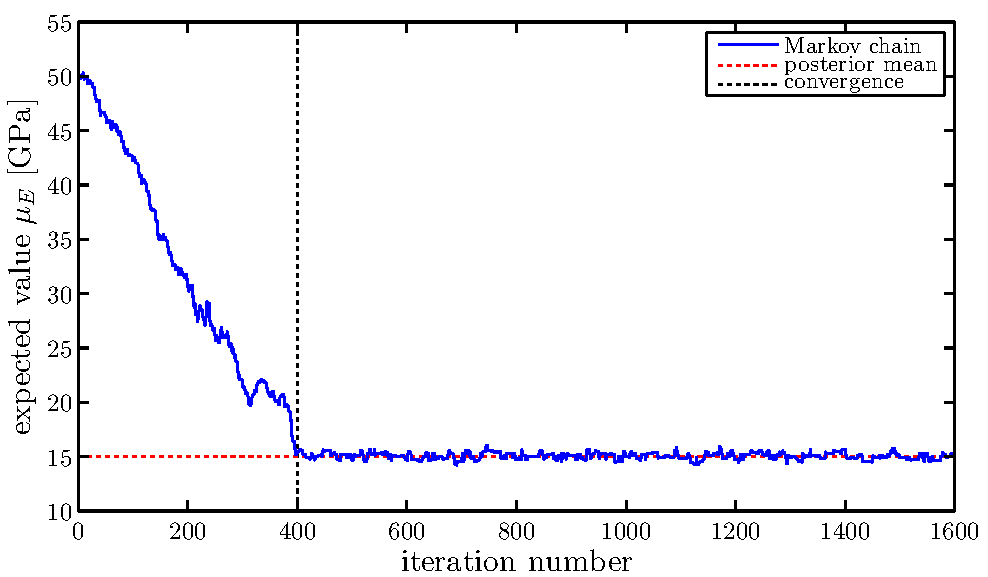
\includegraphics[height=\PEMfigHeight]{fig_PEM_ProbInvChainMean}
    \caption{Convergence of \(\mu_E\).}
    \label{fig:PEM:ProbInv:Chain:Mean}
  \end{subfigure}%
  \begin{subfigure}[b]{0.5\textwidth}
    \centering
    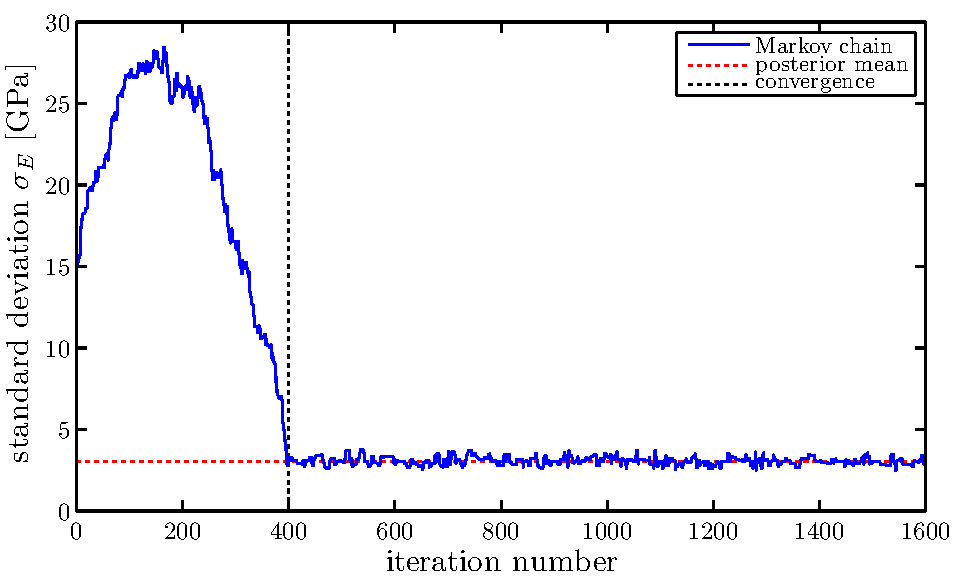
\includegraphics[height=\PEMfigHeight]{fig_PEM_ProbInvChainSigma}
    \caption{Convergence of \(\sigma_E\).}
    \label{fig:PEM:ProbInv:Chain:Sigma}
  \end{subfigure}%
  \caption[Trace plots of a converging Markov chain]{Trace plots of a converging Markov chain.
           For \(n=100\) the converging Markov chain is shown for \(\mu_E\) in \subref{fig:PEM:ProbInv:Chain:Mean} and for \(\sigma_E\) in \subref{fig:PEM:ProbInv:Chain:Sigma}.
           Being initialized at \(\mu_E^{(0)}=\unit[50]{GPa}\) and \(\sigma_E^{(0)}=\unit[15]{GPa}\) the Markov chain converges within ca.\ \(400\) MCMC iterations.
           In equilibrium the Markov chain samples the posterior around its mean.
           }
  \label{fig:PEM:ProbInv:Chains}
\end{figure}
\par % AUTOCORRELATION
In \cref{fig:PEM:ProbInv:ACF} the MCMC sample autocorrelations are plotted for the QoI \((\mu_E,\sigma_E)\) and for an intermediate variable \(E_i\) with \(i=1\).
It can be seen how the autocorrelation function (ACF) drops until it becomes indistinguishable from zero.
This behavior governs the quality of the sample as a posterior representative.
Especially the ACF of \(E_i\) shown in \cref{fig:PEM:ProbInv:ACF:Param} motivates more efficient updating schemes in future research.
% AUTOCORRELATION
\begin{figure}[ht]
  \centering
  % MEAN HYPERPARAMETER
  \begin{subfigure}[b]{0.33\textwidth}
    \centering
    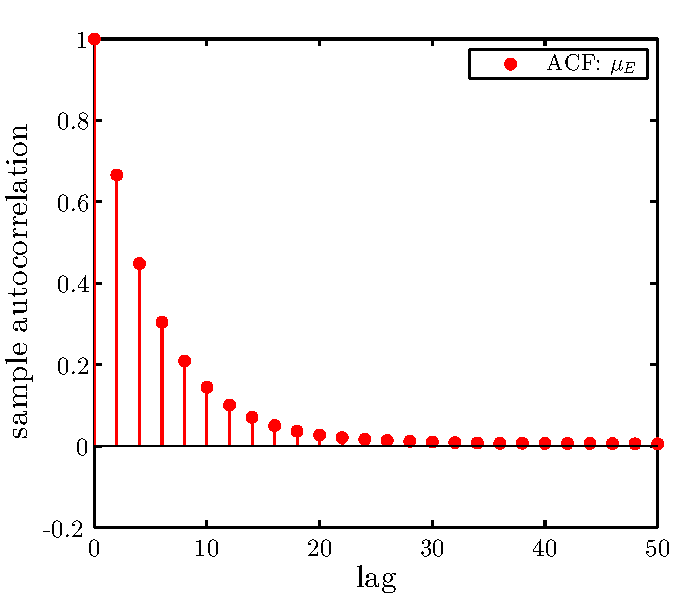
\includegraphics[height=\PEMfigHeight]{fig_PEM_ProbInvACFMean}
    \caption{Autocorrelation of \(\mu_E\).}
    \label{fig:PEM:ProbInv:ACF:Mean}
  \end{subfigure}%
  % SIGMA HYPERPARAMETER
  \begin{subfigure}[b]{0.33\textwidth}
    \centering
    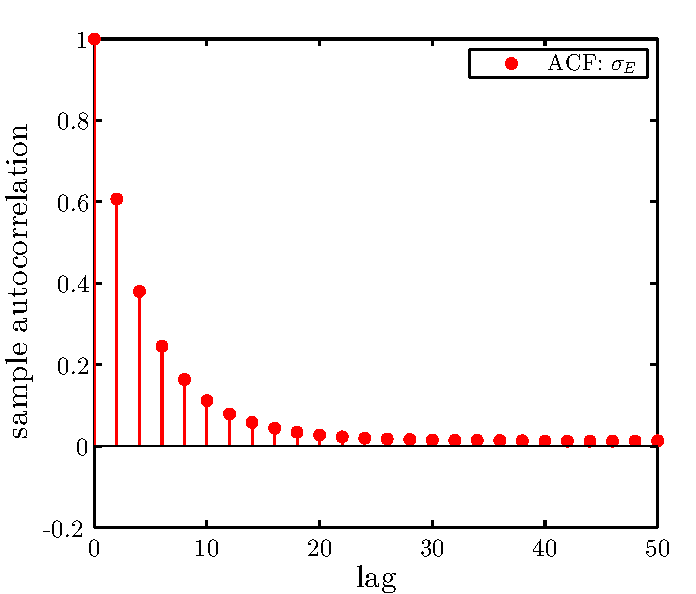
\includegraphics[height=\PEMfigHeight]{fig_PEM_ProbInvACFSigma}
    \caption{Autocorrelation of \(\sigma_E\).}
    \label{fig:PEM:ProbInv:ACF:Sigma}
  \end{subfigure}%
  % INDIVIDUAL PARAMETER
  \begin{subfigure}[b]{0.33\textwidth}
    \centering
    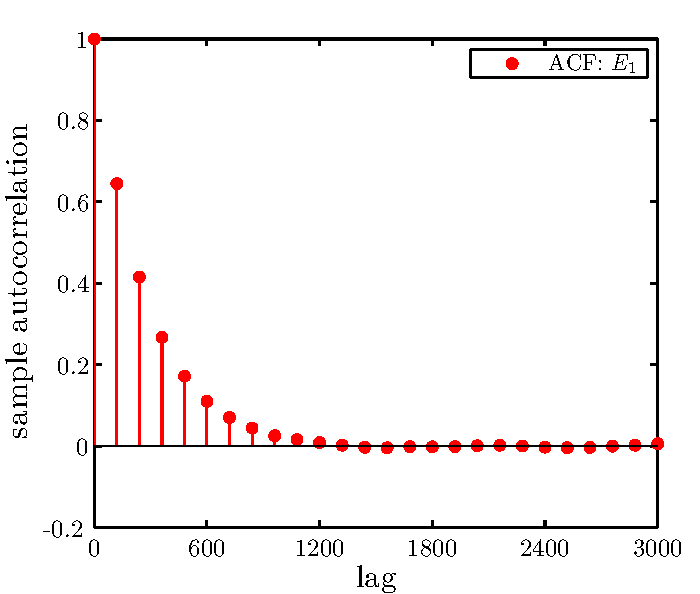
\includegraphics[height=\PEMfigHeight]{fig_PEM_ProbInvACFParam}
    \caption{Autocorrelation of \(E_1\).}
    \label{fig:PEM:ProbInv:ACF:Param}
  \end{subfigure}%
  \caption[Sample autocorrelation functions]{Sample autocorrelation functions.
           For a run with \(n=100\) the MCMC sample autocorrelation function is plotted for \(\mu_E\) in \subref{fig:PEM:ProbInv:ACF:Mean},
           for \(\sigma_E\) in \subref{fig:PEM:ProbInv:ACF:Sigma} and for \(E_1\) in \subref{fig:PEM:ProbInv:ACF:Param}.
           The sample autocorrelation determines the effective MCMC sample size.
           }
  \label{fig:PEM:ProbInv:ACF}
\end{figure}

\subsubsection{Results: Posterior marginals}
% ANALYZED DATA
We analyze the data \(\tuple{\bm{v}_i}_{1\leq i \leq 100}\) as well as its subconfigurations \(\tuple{\bm{v}_i}_{1 \leq i \leq 10}\), \(\tuple{\bm{v}_i}_{1\leq i \leq 20}\) and \(\tuple{\bm{v}_i}_{1\leq i \leq 50}\).
This allows to assess how the number of experiments \(n\) influences the identification of the QoI.
% MCMC ITERATIONS
For each of the runs \(N=10^7\) MCMC iterations are performed.
% BURN-IN
As a general rule we discard the initial \(\unit{1}{\%}\) of the total number of iterations of each Markov chain as a burn-in period.
% COMPUTATION TIME
The total algorithm runtime adds up to \(t=\unit[3.85]{h}\) for \(n=10\) and to \(t=\unit[4.66]{h}\) for \(n=100\).
% POSTERIOR MARGINALS
The resulting posterior marginals of \(\mu_E\) and \(\sigma_E\) are shown in \cref{fig:PEM:ProbInv:Marginals}.
% TABLE
A statistical summary of these marginals can be found in \cref{tab:PEM:ProbInf:Summary}, where the mean, mode, standard deviation (SD) and coefficient of variation (CV) are listed.
% REMARKS
With increasing number of processed experiments \(n\),
Bayesian point estimates (mean, mode) approach the true values \(\mu_E = \unit[15]{GPa}\) and \(\sigma_E = \unit[3]{GPa}\) while measures of estimation uncertainty (SD, CV) expectedly decrease.
% MARGINAL POSTERIORS
\begin{figure}[ht]
  \centering
  \begin{subfigure}[b]{0.5\textwidth}
    \centering
    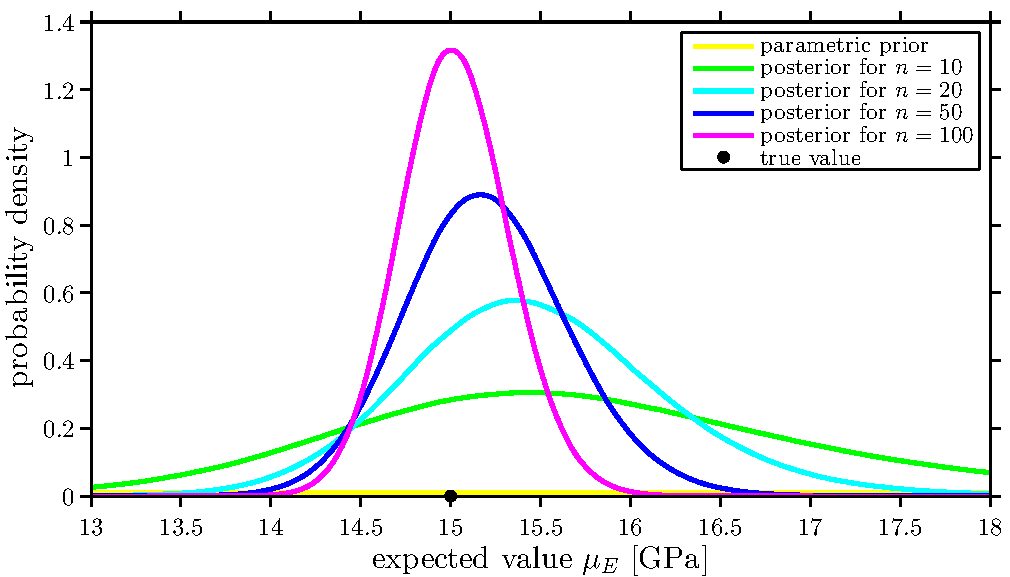
\includegraphics[height=\PEMfigHeight]{fig_PEM_ProbInvPostMean}
    \caption{Posterior marginal of \(\mu_E\).}
    \label{fig:PEM:ProbInv:Post:Mean}
  \end{subfigure}%
  \begin{subfigure}[b]{0.5\textwidth}
    \centering
    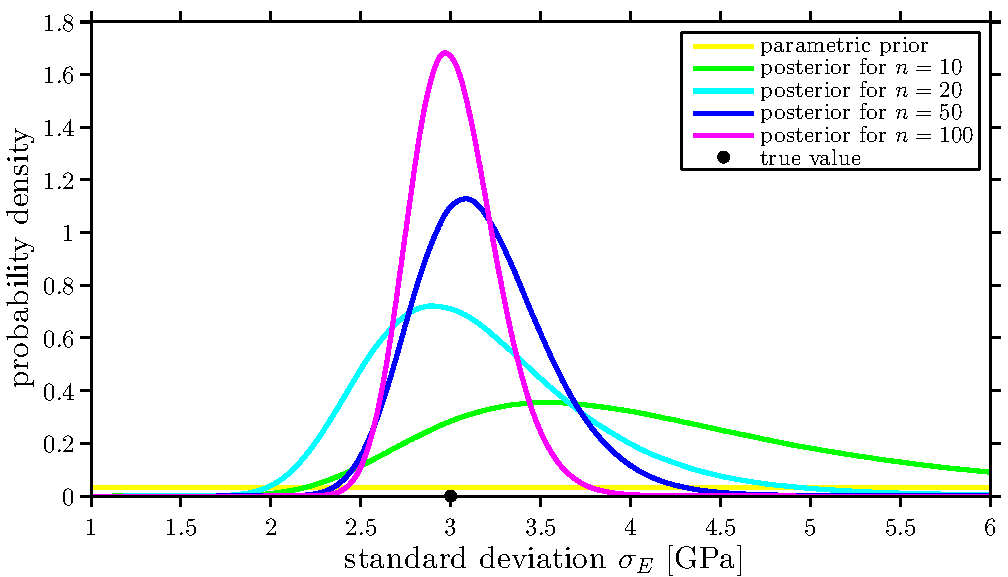
\includegraphics[height=\PEMfigHeight]{fig_PEM_ProbInvPostSigma}
    \caption{Posterior marginal of \(\sigma_E\).}
    \label{fig:PEM:ProbInv:Post:Sigma}
  \end{subfigure}%
  \caption[Posterior marginals of the QoI]{Posterior marginals of the QoI.
           Corresponding to various numbers of experiments \(n\), the marginal posterior densities of \(\mu_E\) and \(\sigma_E\)
           are shown in \subref{fig:PEM:ProbInv:Post:Mean} and \subref{fig:PEM:ProbInv:Post:Sigma}, respectively.
           For increasing \(n\), the posterior uncertainty in estimating the QoI \(\bm{\theta}_E = (\mu_E,\sigma_E)\)
           with \(\mu_E=\unit[15]{GPa}\) and \(\sigma_E = \unit[3]{GPa}\) steadily decreases.
          }
  \label{fig:PEM:ProbInv:Marginals}
\end{figure}
% TABLE: PROBABILISTIC INVERSION
\begin{table}[ht]
  \caption[Summary of the QoI posterior marginals]{Summary of the QoI posterior marginals.}
  \label{tab:PEM:ProbInf:Summary}
  \centering
  \begin{tabular}{lcccccccccc}
    \toprule
    & \phantom{} & \multicolumn{3}{c}{\(\mu_E\) \(\lbrack\unit[]{GPa}\rbrack\)} & \(\lbrack \unitless \rbrack\)
    & \phantom{} & \multicolumn{3}{c}{\(\sigma_E\) \(\lbrack\unit[]{GPa}\rbrack\)} & \(\lbrack \unitless \rbrack\) \\
    \cmidrule{3-6} \cmidrule{8-11}
    && Mean & Mode & SD & CV && Mean & Mode & SD & CV \\
    \midrule
    \(n=10\)  && \(15.98\) & \(15.43\) & \(2.06\) & \(0.13\) && \(4.73\) & \(3.54\) & \(3.55\) & \(0.75\) \\
    \(n=20\)  && \(15.48\) & \(15.36\) & \(0.74\) & \(0.05\) && \(3.18\) & \(2.90\) & \(0.65\) & \(0.20\) \\
    \(n=50\)  && \(15.20\) & \(15.17\) & \(0.46\) & \(0.03\) && \(3.17\) & \(3.08\) & \(0.37\) & \(0.12\) \\
    \(n=100\) && \(15.02\) & \(15.00\) & \(0.30\) & \(0.02\) && \(3.02\) & \(2.97\) & \(0.24\) & \(0.08\) \\
    \bottomrule
  \end{tabular}
\end{table}

\subsubsection{Results: Two-dimensional posteriors}
% 2D POSTERIOR
Showing posterior marginals may hide possibly existing dependency structures or the lack thereof.
Those constitute a substantial result of Bayesian data analysis, though.
Hence \cref{fig:PEM:ProbInv:2DPosterior} shows two-dimensional posteriors where interesting correlation properties were discovered.
% HYPERPARAMETERS
The two-dimensional posterior of \((\mu_E,\sigma_E)\) is plotted in \cref{fig:PEM:ProbInv:2DPosterior:MeanSigma}.
According to the posterior probability model these two parameters are correlated with a linear Pearson coefficient of correlation \(r_{\mu_E,\sigma_E}=0.40\).
Note that these parameters were assumed to be independent in accord with their prior model.
% JOINT POSTERIOR
The joint posterior \cref{eq:PEM:ProbInv:JointPosterior} can also feature a correlation between hyperparameters and experiment-specific parameters.
In \cref{fig:PEM:ProbInv:2DPosterior:MeanParam,fig:PEM:ProbInv:2DPosterior:ParamParam} the two-dimensional posteriors of \((\mu_E,E_i)\) and \((E_{j},E_{i})\) with \(i=50\) and \(j=75\) are imaged.
% 2D POSTERIORS
\begin{figure}[ht]
  \centering
  \begin{subfigure}[b]{0.33\textwidth}
    \centering
    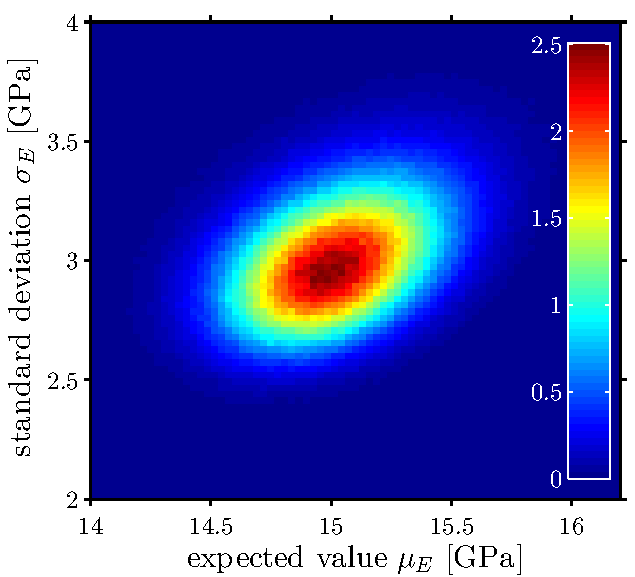
\includegraphics[height=\PEMfigHeight]{fig_PEM_ProbInvPost2DMeanSigma}
    \caption{2D posterior of \((\mu_E,\sigma_E)\).}
    \label{fig:PEM:ProbInv:2DPosterior:MeanSigma}
  \end{subfigure}%
  \begin{subfigure}[b]{0.33\textwidth}
    \centering
    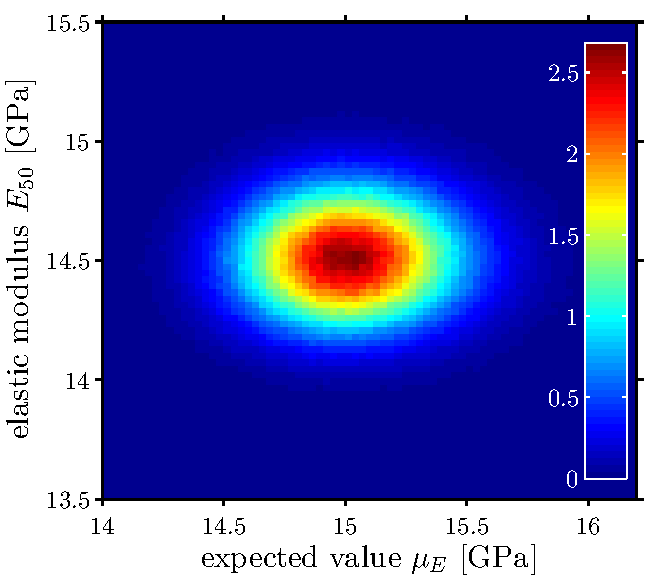
\includegraphics[height=\PEMfigHeight]{fig_PEM_ProbInvPost2DMeanParam}
    \caption{2D posterior of \((\mu_E,E_{50})\).}
    \label{fig:PEM:ProbInv:2DPosterior:MeanParam}
  \end{subfigure}%
  \begin{subfigure}[b]{0.33\textwidth}
    \centering
    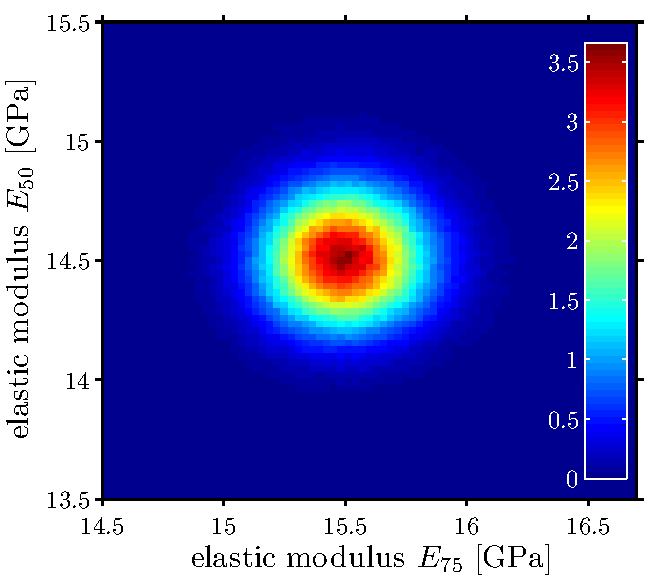
\includegraphics[height=\PEMfigHeight]{fig_PEM_ProbInvPost2DParamParam}
    \caption{2D posterior of \((E_{75},E_{50})\).}
    \label{fig:PEM:ProbInv:2DPosterior:ParamParam}
  \end{subfigure}%
  \caption[2D posteriors of \((\mu_E,\sigma_E)\), \((\mu_E,E_{50})\) and \((E_{75},E_{50})\)]{2D posteriors of \((\mu_E,\sigma_E)\), \((\mu_E,E_{50})\) and \((E_{75},E_{50})\).
           The two-dimensional posteriors of \((\mu_E,\sigma_E)\), \((\mu_E,E_{50})\) and \((E_{75},E_{50})\) are shown.
           Being priorly independent the components \(\mu_E\) and \(\sigma_E\) are seen to be correlated a posteriori.
           The linear Pearson coefficient of correlation amounts to \(r_{\mu_E,\sigma_E}=0.40\).
           }
  \label{fig:PEM:ProbInv:2DPosterior}
\end{figure}

%%%%%%%%%%%%%%%%%%%%%%%%%%%%%%%%%%%%%%%%%%%%%%%%%%%%%%%%%%%%%%%%%%%%%%%%%%%%%%%%%%%%%%%%%%%%%%%%%%%%%%%%%%%%%%%%%%%%%%%%%%%%%%%%%%%%%%%%%%%%%%%%%%%%%%%%%%%%%%%%%%%%%%%%%%%%%%%%%%%%%%%%%
\subsection{Residual calibration} \label{sec:PEM:CaseStudies:ResCal}
%%%%%%%%%%%%%%%%%%%%%%%%
% RESIDUAL CALIBRATION %
%%%%%%%%%%%%%%%%%%%%%%%%
There are situations where the strong assumption of known residual variances \(\bm{\Sigma}_i = \sigma_i^2 \bm{I}_3\) is somewhat restrictive.
Thus we generalize multilevel inversion as in \cref{sec:PEM:CaseStudies:ProbInv} by treating \(\sigma_{\mathcal{E}} \equiv \sigma_i\) as a global unknown.
% PRIOR MODEL
In units of \(\unit[]{mm}\) the corresponding parametric prior is set to a uniform distribution \(\pi(\sigma_{\mathcal{E}}) = \mathcal{U}(0,0.5)\).
% EXPERIMENTAL SETUP
Otherwise the experimental setup of probabilistic inversion is used.
\par % INFERENTIAL MECHANISM
The standard deviation \(\sigma_{\mathcal{E}}\) of the residual model \(\mathcal{N}(\bm{\varepsilon}_i \cond \bm{0},\sigma_{\mathcal{E}}^2 \bm{I}_3)\)
is introduced as an extra unknown in the model \cref{eq:PEM:ProbInv:Model} and in the posterior \cref{eq:PEM:ProbInv:JointPosterior}.
% PRIOR & POSTERIOR
Consequently the joint prior is given as \(\pi(\tuple{E_i},\mu_E,\sigma_E,\sigma_{\mathcal{E}}) = \pi(\sigma_{\mathcal{E}}) \, \pi(\mu_E) \, \pi(\sigma_E) \prod_{i=1}^n \mathcal{LN}(E_i \cond \mu_E,\sigma_E)\).
For the joint likelihood function one has \(\mathcal{L}(\tuple{E_i},\sigma_{\mathcal{E}} \distparam \tuple{\bm{v}_i}) = \prod_{i=1}^n \mathcal{N}(\bm{v}_i \allowbreak \cond \mathcal{M}(E_i,F_i,\bm{l}_i,\bm{s}_i),\sigma_{\mathcal{E}}^2 \bm{I}_3)\).
Brought together this leads to a joint posterior density that has the shape
\(\pi(\tuple{E_i},\mu_E,\sigma_E, \allowbreak \sigma_{\mathcal{E}} \cond \tuple{\bm{v}_i}) \propto \mathcal{L}(\tuple{E_i},\sigma_{\mathcal{E}} \distparam \tuple{\bm{v}_i}) \, \pi(\tuple{E_i},\mu_E,\sigma_E,\sigma_{\mathcal{E}})\).
\par % MCMC
We sample from this posterior by appending a block for the additional unknown \(\sigma_{\mathcal{E}}\) in the MCMC updating scheme.
In order to assess the influence of the amount of data on the final results, independent runs are performed for \(n = 10\), \(20\), \(50\) and \(100\).
% RESULTS
In \cref{fig:PEM:ResCal:Post:Mean} the relevant posterior marginals for the inference of the residual model \(\sigma_{\mathcal{E}}\) are shown.
A short summary of the these marginals is provided in \cref{tab:PEM:ResCal:Summary}.
% OBSERVATION & INTERPRETATION
The higher the number of analyzed experiments \(n\), the better the true value \(\sigma_{\mathcal{E}} = \unit[0.1]{mm}\) has been revealed.
This proves that one can indeed estimate the parameters of the prediction error model in the context of multilevel calibration.
If this is not of interest for its own sake, it still avoids the requirement of perfect knowledge of the error variance.
% PROBABILISTIC INVERSION
In addition we observed that introducing an uncertainty in the residual model hardly affects the inference of the QoI in probabilistic inversion.
% MARGINAL POSTERIORS: FIGURE & SUMMARY
\begin{figure}[ht]
  \centering
  % MARGINAL POSTERIORS: RESIDUAL SIGMA
  \begin{minipage}[c]{0.52\textwidth}
    \centering
    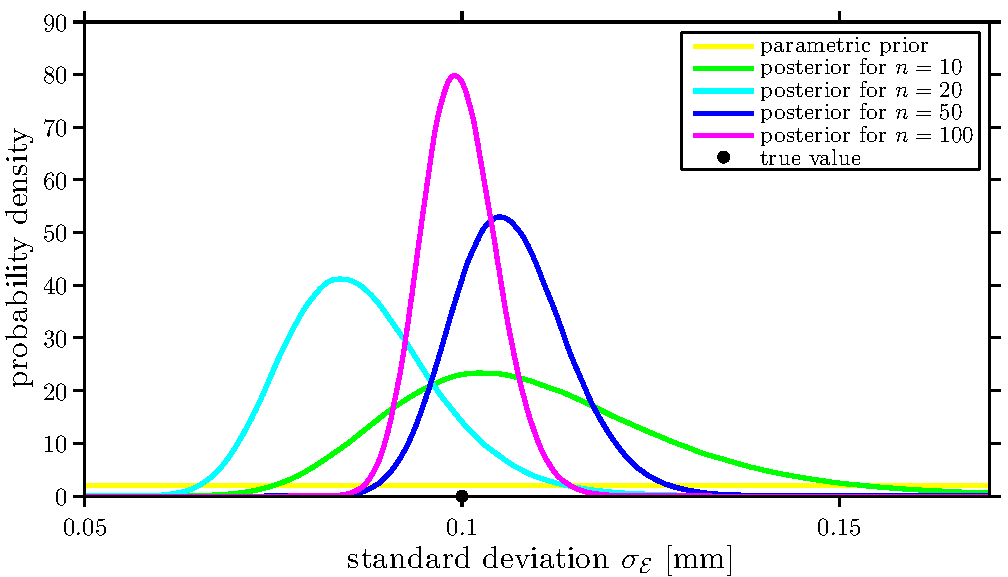
\includegraphics[height=\PEMfigHeight]{fig_PEM_ResCalPostResidualSigma}
    \captionof{figure}[Posterior marginals of \(\sigma_{\mathcal{E}}\)]{Posterior marginals of \(\sigma_{\mathcal{E}}\).
    The marginal posterior of \(\sigma_{\mathcal{E}}\) is shown for different numbers of data \(n\).
    }
    \label{fig:PEM:ResCal:Post:Mean}
  \end{minipage}%
  \hfill%
  % TABLE: RESIDUAL CALIBRATION
  \begin{minipage}[c]{0.46\textwidth}
    \captionof{table}[Summary of the \(\sigma_{\mathcal{E}}\)-marginals]{Summary of the \(\sigma_{\mathcal{E}}\)-marginals.}
    \label{tab:PEM:ResCal:Summary}
    \centering
    \begin{tabular}{lrrrrr}
      \toprule
      & \phantom{} & \multicolumn{3}{c}{\(\sigma_{\mathcal{E}}\) \(\lbrack\unit[10^{-5}]{m}\rbrack\)} & \multicolumn{1}{c}{\(\lbrack \unitless \rbrack\)} \\
      \cmidrule{3-6}
      && \multicolumn{1}{c}{Mean} & \multicolumn{1}{c}{Mode} & \multicolumn{1}{c}{SD} & \multicolumn{1}{c}{CV} \\
      \midrule
      \(n=10\)  && \(11.00\) & \(10.23\) & \(1.90\) & \(0.17\) \\
      \(n=20\)  && \(8.68\)  & \(8.38\)  & \(1.01\) & \(0.12\) \\
      \(n=50\)  && \(10.65\) & \(10.50\) & \(0.77\) & \(0.07\) \\
      \(n=100\) && \(9.97\)  & \(9.90\)  & \(0.50\) & \(0.05\) \\
      \bottomrule
    \end{tabular}
  \end{minipage}%
\end{figure}

%%%%%%%%%%%%%%%%%%%%%%%%%%%%%%%%%%%%%%%%%%%%%%%%%%%%%%%%%%%%%%%%%%%%%%%%%%%%%%%%%%%%%%%%%%%%%%%%%%%%%%%%%%%%%%%%%%%%%%%%%%%%%%%%%%%%%%%%%%%%%%%%%%%%%%%%%%%%%%%%%%%%%%%%%%%%%%%%%%%%%%%%%
\subsection{Uncertain conditions} \label{sec:PEM:CaseStudies:AddPres}
%%%%%%%%%%%%%%%%%%%%%%%
% ADDITIONAL NUISANCE %
%%%%%%%%%%%%%%%%%%%%%%%
In the following we describe an experimental situation where the inference of the QoI \(\bm{\theta}_E\) is hampered by additional uncertainties in the experimental conditions.
Experimental conditions are formally treated as nuisance parameters with prescribed uncertainties.
More specifically, we do not assume that the loads \(F_i\) are perfectly known anymore.
In contrast, we assume that they are \(\bm{\zeta}_i\)-type variables, i.e.\ they are uncertain yet they follow a known distribution.
% EXPERIMENTAL SITUATION
This represents a well-known situation where the loads \(F_i\) that the testing machine actually applies can only be imprecisely adjusted.
In fact, while a targeted load in each experiment is chosen, the physically realized load \(F_i\) may be uncertain.
This is accounted for by a prescribed distribution \(\mathcal{N}(F_i \distparam \mu_{F_i},\sigma_{F_i}^2)\)
where \(\mu_{F_i}\) is the targeted load and \(\sigma_{F_i}\) represents the degree of uncertainty that is inherent to the test machinery.
\par % NUMERICAL SETUP
The setup for conducting a numerical experiment is similar to the one specified in \cref{sec:PEM:CaseStudies:ProbInv}.
For \(n=50\) beams we set the beam dimensions \(\bm{l}_i\) and measurement positions \(\bm{s}_i\) as before.
Elastic moduli \(E_i\) are randomly drawn from \(\mathcal{LN}(E_i \cond \mu_E,\sigma_E)\) as previously detailed.
In contrast to plain probabilistic inversion, for \(i=1,\ldots,n\) experiment-specific loads \(F_i\) are independently sampled from
normal distributions \(\mathcal{N}(F_i \distparam \mu_{F_i},\sigma_{F_i}^2)\) with \(\mu_{F_i} = \unit[30]{kN}\) and \(\sigma_{F_i} = \unit[3]{kN}\).
This equates to a coefficient of variation \(c_{F_i} = \unit[10]{\%}\).
% COMMENTS
Note that such a high degree of uncertainty is unlikely to be encountered in a real-case experiment.
It is used here to accentuate the results presented below, though.
% TREATED AS UNKNOWNS
The realized loads \(F_i\) will be treated as unknowns whereas the hyperparameters \(\bm{\theta}_{F_i} = (\mu_{F_i},\sigma_{F_i})\), i.e.\ the targeted load and its uncertainty, will be treated as knowns.
% PSEUDO MEASUREMENTS
In accordance with \cref{eq:PEM:Beams:AlgebraicFormula} synthetic measurements \(\bm{v}_i = \perfect{\bm{v}}_i + \bm{\varepsilon}_i\) are generated again.
% HYPERPRIORS
The prior distribution \(\pi(\bm{\theta}_E) = \pi(\mu_E) \, \pi(\sigma_E)\) is also chosen as previously stated.
\par % SUMMARY
The problem of probabilistic inversion under additional prescribed nuisance reads as follows.
The hyperparameters \(\bm{\theta}_{\bm{X}} \equiv \bm{\theta}_E\) are the QoI
whereas experiment-specific unknowns \(\tuple{\bm{x}_i} \equiv \tuple{E_i}\) and \(\tuple{\bm{\zeta}_i} \equiv \tuple{F_i}\) are considered nuisance.
With measurements \(\tuple{\bm{y}_i} \equiv \tuple{\bm{v}_i}\) the QoI can be inferred.
Experimental-specific knowns consist of the hyperparameters \(\tuple{\bm{\theta}_{\bm{Z}_i}} \equiv \tuple{\bm{\theta}_{F_i}}\),
the experimental conditions \(\tuple{\bm{d}_i} \equiv \tuple{(\bm{l}_i,\bm{s}_i)}\) and the residual covariances \(\tuple{\bm{\Sigma}_i}\).
Parametric Bayesian prior knowledge is given by \(\pi_{\bm{\Theta}_{\bm{X}}}(\bm{\theta}_{\bm{X}}) \equiv \pi(\bm{\theta}_E)\)
whereas \(f_{\bm{X} \cond \bm{\Theta}_{\bm{X}}} (\bm{x}_i \cond \bm{\theta}_{\bm{X}}) \equiv \mathcal{LN}(E_i \cond \mu_E,\sigma_E)\) and 
\(f_{\bm{Z}}(\bm{\zeta}_i \distparam \bm{\theta}_{\bm{Z}_i}) \equiv \mathcal{N}(F_i \distparam \mu_{F_i},\sigma_{F_i}^2)\) are structural prior distributions.
Within a joint approach a posterior of the form \(\pi( \tuple{\bm{x}_i},\tuple{\bm{\zeta}_i},\bm{\theta}_{\bm{X}} \cond \tuple{\bm{y}_i}) \equiv \pi( \tuple{E_i},\tuple{F_i},\bm{\theta}_E \cond \tuple{\bm{v}_i})\) arises.
Eventually one is interested in the QoI-marginals \( \pi(\bm{\theta}_{\bm{X}} \cond \tuple{\bm{y}_i}) \equiv \pi(\bm{\theta}_E \cond \tuple{\bm{v}_i})\) only.
% DAG
A DAG corresponding to this experimental situation is shown in \cref{fig:PEM:DAG:AddPres}.

\subsubsection{Results: Hyperparameters}
% PROBLEM FORMULATIONS
We sample the joint posterior \(\pi(\tuple{E_i},\tuple{F_i},\bm{\theta}_E \cond \tuple{\bm{v}_i})\) where nuisance variables \(\tuple{F_i}\) are explicitly accounted for.
% BLOCKSWISE MCMC
In a blockwise manner MCMC sweeps are accomplished for \((\mu_E,\sigma_E)\), \(\tuple{E_i}\) and \(\tuple{F_i}\) which constitute different blocks.
Blockwise proposal distributions are again adjusted in order to obtain acceptance rates in between \(\unit[20]{\%}\) and \(\unit[40]{\%}\).
% INITIALIZATION
Each \(F_i\) in the block \(\tuple{F_i}\) is initialized at \(F_i^{(0)} = \mu_{F_i}\), i.e.\ the structural prior mean.
% CONVERGENCE CHECKS
Other than that initialization, convergence checks and burn-in are accomplished as before.
% COMPUTATION TIME
For \(N=10^7\) MCMC iterations the total computation time amounts to \(t=\unit[7.18]{h}\).
% POSTERIOR MARGINALS
The resulting posterior marginals of \(\mu_E\) and \(\sigma_E\) can be seen in \cref{fig:PEM:AddPres:Marginals}.
A statistical summary is provided in \cref{tab:PEM:AddPres:Summary} where the mean, mode, SD and CV of the marginals are itemized.
% MARGINAL POSTERIORS
\begin{figure}[ht]
  \centering
  \begin{subfigure}[b]{0.5\textwidth}
    \centering
    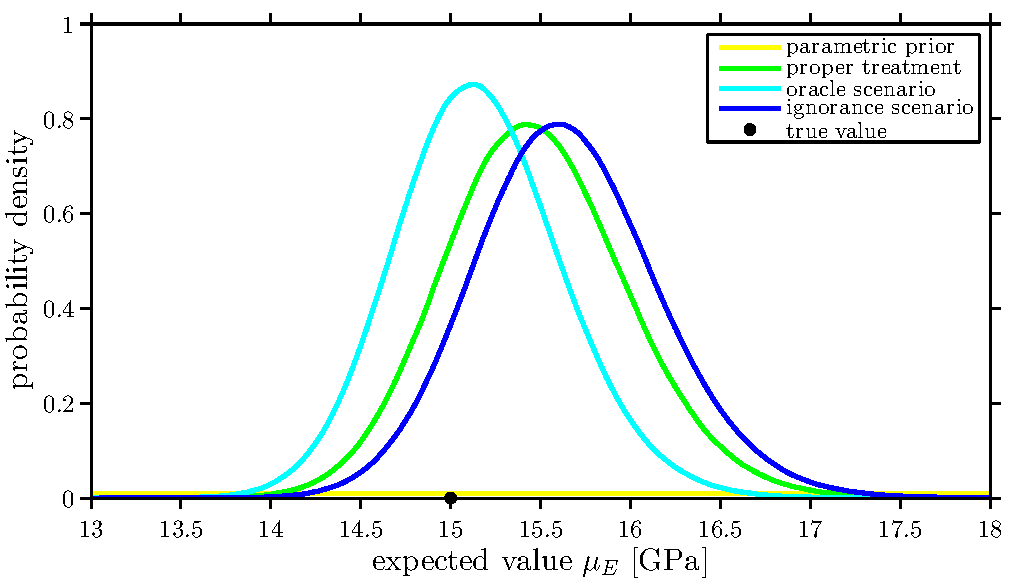
\includegraphics[height=\PEMfigHeight]{fig_PEM_AddPresPostMean}
    \caption{Posterior marginal of \(\mu_E\).}
    \label{fig:PEM:AddPres:Post:Mean}
  \end{subfigure}%
  \begin{subfigure}[b]{0.5\textwidth}
    \centering
    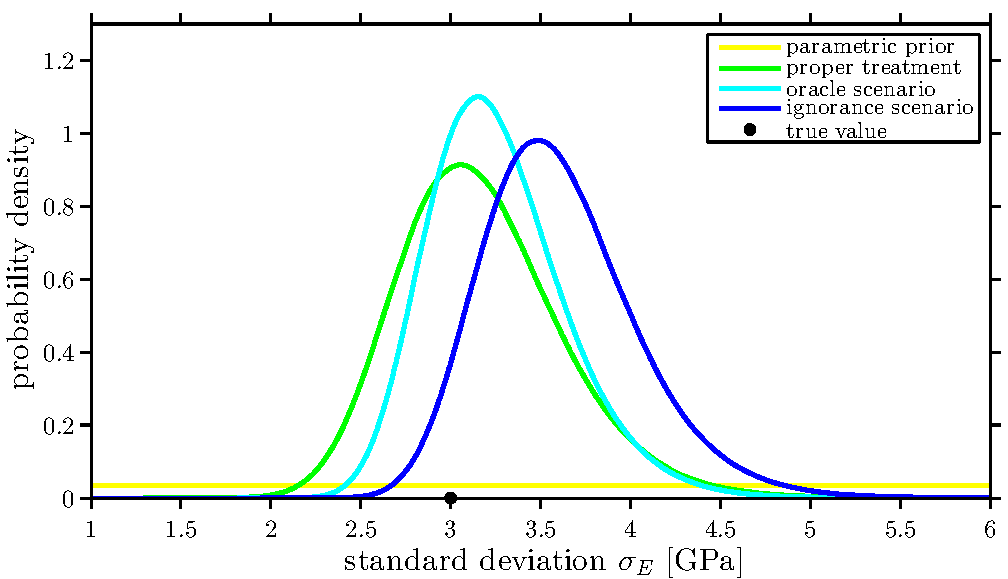
\includegraphics[height=\PEMfigHeight]{fig_PEM_AddPresPostSigma}
    \caption{Posterior marginal of \(\sigma_E\).}
    \label{fig:PEM:AddPres:Post:Sigma}
  \end{subfigure}%
  \caption[Posterior marginals of the QoI]{Posterior marginals of the QoI.
           The marginal posteriors of \(\mu_E\) and \(\sigma_E\) are provided in \subref{fig:PEM:AddPres:Post:Mean} and \subref{fig:PEM:AddPres:Post:Sigma}, respectively.
           Three experimental scenarios are investigated: the proper treatment of the additional uncertainty, 
           an idealized situation where one would precisely know the loads, and the case of a parsimonious model where the uncertainty remains unrecognized.
          }
  \label{fig:PEM:AddPres:Marginals}
\end{figure}
% TABLE: ADDITIONAL PRESCRIPTION
\begin{table}[ht]
  \caption[Summary of the QoI posterior marginals]{Summary of the QoI posterior marginals.}
  \label{tab:PEM:AddPres:Summary}
  \centering
  \begin{tabular}{lcccccccccc}
    \toprule
      & \phantom{} & \multicolumn{3}{c}{\(\mu_E\) \(\lbrack\unit[]{GPa}\rbrack\)} & \(\lbrack \unitless \rbrack\)
      & \phantom{} & \multicolumn{3}{c}{\(\sigma_E\) \(\lbrack\unit[]{GPa}\rbrack\)} & \(\lbrack \unitless \rbrack\) \\
    \cmidrule{3-6} \cmidrule{8-11}
    && Mean & Mode & SD & CV && Mean & Mode & SD & CV \\
    \midrule
    Proper treatment   && \(15.47\) & \(15.41\) & \(0.51\) & \(0.03\) && \(3.17\) & \(3.05\) & \(0.46\) & \(0.14\) \\
    Oracle scenario    && \(15.16\) & \(15.13\) & \(0.47\) & \(0.03\) && \(3.26\) & \(3.15\) & \(0.39\) & \(0.12\) \\
    Ignorance scenario && \(15.65\) & \(15.60\) & \(0.52\) & \(0.03\) && \(3.61\) & \(3.51\) & \(0.43\) & \(0.12\) \\
    \bottomrule
  \end{tabular}
\end{table}
\par % POSTERIOR SIGNIFICANCE
We try to assess the impact of the uncertainty that had been introduced in the loads \(F_i\) on the estimation of the QoI \(\bm{\theta}_E = (\mu_E,\sigma_E)\).
To that end we pursue the following two strategies.
% IDEALIZED SITUATION
First of all we estimate the QoI while treating the realized loads \(F_i\) as if they were part of the experiment-specific knowns \(\bm{d}_i\).
This ``what-if'' or ``oracle'' scenario actually describes the hypothetical situation that we met in plain probabilistic inversion.
It does not describe the realistic scenario of uncertain conditions \(\bm{\zeta}_i\) that we are actually investigating.
Yet this way of proceeding sheds light on how the prescribed uncertainty in the loads affects the inference of the QoI.
% INTERPRETATION
For \(N=10^7\) and \(t=\unit[4.33]{h}\) the results to probabilistic inversion are added to \cref{fig:PEM:AddPres:Marginals}.
With respect to this idealized situation, one can reassess the previous results of properly treating the loads as uncertain.
The introduction of the uncertainty in the loads had actually shifted the posterior modes and raised the level of estimation uncertainty accordingly.
\par % UNCERECOGNIZED UNCERTAINTY
Second of all we investigate the case that the uncertainty \(\mathcal{N}(F_i \distparam \mu_{F_i},\sigma_{F_i}^2)\) in the applied loads \(F_i\) is simply disregarded.
Either it has not been recognized by mistake or it has been intentionally dropped by making simplifying assumptions in favor of a parsimonious model.
% MISTREATMENT
Rather than treating the loads as belonging to the unknowns \(\bm{\zeta}_i\), we erroneously treat them as such experimental conditions \(\erroneous{\bm{d}}_i\) that only approximately describe the prevailing conditions \(\bm{d}_i\).
While the data has been created under \(\bm{d}_i\), data analysis is carried out under \(\erroneous{\bm{d}}_i\).
% EXPERIMENTAL SITUATION
This describes a situation where the experimenter targets a load \(\erroneous{F}_i = \mu_{F_i}\), but the testing machine actually realizes \(F_i\).
If this uncertainty \(\mathcal{N}(F_i \distparam \mu_{F_i},\sigma_{F_i}^2)\) is not accounted for or not recognized at all,
the analyst will accomplish inference under the spurious assumption that the loads had taken on their targeted values \(\erroneous{F}_i\) during experiment execution.
% RESULTS & INTERPRETATION
For \(N=10^7\) and \(t=\unit[3.75]{h}\) the resulting posteriors are added to \cref{fig:PEM:AddPres:Marginals}.
Our interpretation is that dropping the uncertainty of \(F_i\) corrupts the estimation of the QoI and results in misleading estimates of posterior uncertainty,
whereas the proper treatment of all uncertainties yields results that are closer to the idealized ``oracle'' scenario.

\subsubsection{Results: Intermediate variables}
\par % FURTHER INSIGHTS
Sampling the joint posterior \(\pi(\tuple{E_i},\tuple{F_i},\bm{\theta}_E \cond \tuple{\bm{v}_i})\) of the entirety of unknowns provides further interesting insights.
% POSTERIOR OF THE LOADS
Apart from the QoI-marginals one can examine the posterior model of experiment-specific loads \(F_i\), notwithstanding that they are considered nuisance.
\cref{fig:PEM:AddPres:Posteriors} contains two different posteriors involving some \(F_i\).
In \cref{fig:PEM:AddPres:Post:1DLoad} the posterior marginal of a pinpoint load \(F_i\) is shown for \(i=23\).
The identification of specifically applied loads \(F_i\) is subject to rather high levels of posterior uncertainty.
% IDENTIFIABILITY
This is an issue of statistical identifiability.
When both \(E_i\) and \(F_i\) are uncertain and various combinations of these can explain the observation \(\bm{v}_i\) equally well, then those combinations \((E_i,F_i)\) cannot be distinguished a posteriori.
Of course, the reason is that only the ratio \(F_i/E_i\) in \cref{eq:PEM:Beams:AlgebraicFormula} can be identified.
% POSTERIOR CORRELATION
It is therefore interesting to investigate the posterior correlation between the load \(F_i\) and the modulus \(E_i\) of an experiment \(i\).
The two-dimensional posterior of \((E_i,F_i)\) for \(i=20\) that is shown in \cref{fig:PEM:AddPres:Post:2DMeanLoad} serves as an example.
Posterior mass is assigned to suitable parameter constellations \((E_i,F_i)\) that well-explain the measurement \(\bm{v}_i\).
As expected the posterior is strongly correlated with a linear coefficient of correlation \(r_{F_{20},E_{20}} = 0.99\).
% POSTERIORS: ADDITIONAL PRESCRIPTION
\begin{figure}[ht]
  \centering
  % MARGINAL POSTERIOR: APPLIED LOAD
  \begin{subfigure}[b]{0.5\textwidth}
    \centering
    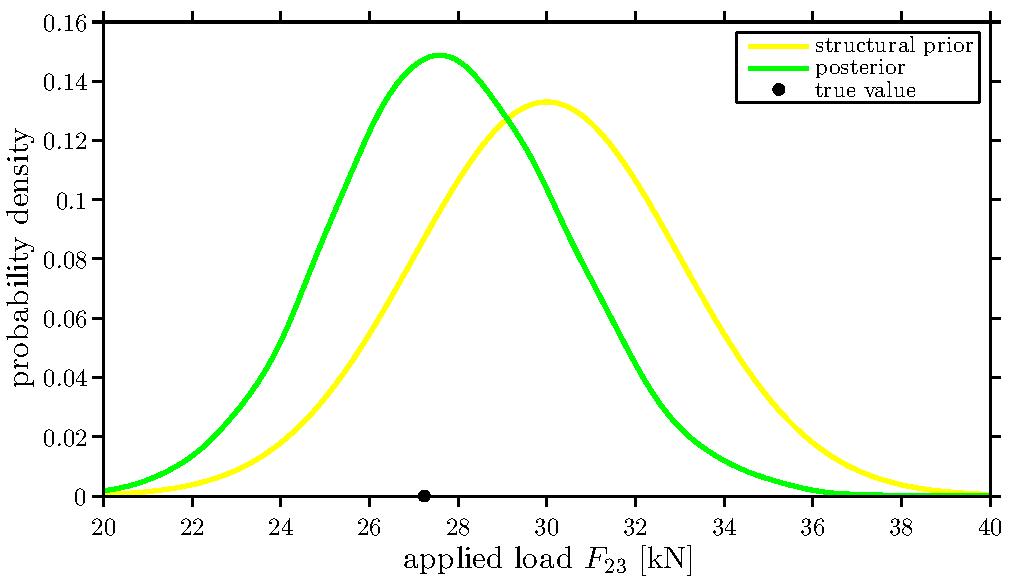
\includegraphics[height=\PEMfigHeight]{fig_PEM_AddPresPostLoad}
    \caption{Posterior marginal of \(F_{23}\).}
    \label{fig:PEM:AddPres:Post:1DLoad}
  \end{subfigure}%
  % 2D POSTERIOR: LOAD-MODULUS
  \begin{subfigure}[b]{0.5\textwidth}
    \centering
    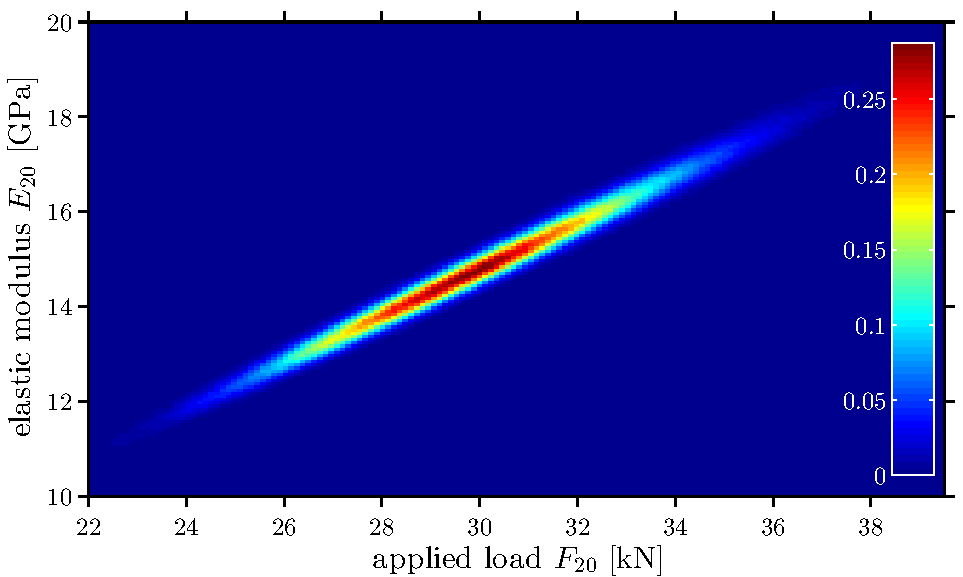
\includegraphics[height=\PEMfigHeight]{fig_PEM_AddPresPost2DLoadParam}
    \caption{2D posterior of \((F_{20},E_{20})\).}
    \label{fig:PEM:AddPres:Post:2DMeanLoad}
  \end{subfigure}%
  \caption[Posteriors of intermediate variables]{Posteriors of intermediate variables.
           In \subref{fig:PEM:AddPres:Post:1DLoad} the posterior marginal of \(F_{23}\) and its structural prior
           \(\mathcal{N}(F_{23} \distparam \mu_{F_{23}},\sigma_{F_{23}}^2)\) with \(\mu_{F_{23}}=\unit[30]{kN}\) and \(\sigma_{F_{23}}=\unit[3]{kN}\) are shown.
           The posterior is centered around the actual value \(F_{23} = \unit[27.24]{kN}\).
           The two-dimensional posterior of \((F_{20},E_{20})\) with \(r_{F_{20},E_{20}} = 0.99\) is shown in \subref{fig:PEM:AddPres:Post:2DMeanLoad}.
          }
  \label{fig:PEM:AddPres:Posteriors}
\end{figure}

%%%%%%%%%%%%%%%%%%%%%%%%%%%%%%%%%%%%%%%%%%%%%%%%%%%%%%%%%%%%%%%%%%%%%%%%%%%%%%%%%%%%%%%%%%%%%%%%%%%%%%%%%%%%%%%%%%%%%%%%%%%%%%%%%%%%%%%%%%%%%%%%%%%%%%%%%%%%%%%%%%%%%%%%%%%%%%%%%%%%%%%%%
\subsection{Borrowing strength} \label{sec:PEM:CaseStudies:CombInf}
%%%%%%%%%%%%%%%%%%%%%%
% BORROWING STRENGTH %
%%%%%%%%%%%%%%%%%%%%%%
As pointed out in \cref{sec:PEM:CombInf}, Bayesian multilevel modeling allows for ``optimal combination of information'' or ``borrowing strength''.
Here we demonstrate this inferential mechanism and investigate its underlying flow of information for the previous application example.
% QOI / NUISANCE
The Bayesian model of probabilistic inversion \cref{eq:PEM:ProbInv:Model} is considered.
However, as opposed to probabilistic inversion we declare experiment-specific elastic moduli \(\tuple{E_i}\) as the QoI whereas the hyperparameters \(\bm{\theta}_E\) are considered nuisance.
Herein we highlight the optimal inference of a single \(E_{\analyzed}\) for some \(\analyzed \in \{1,\ldots,n\}\).
\par % EXPERIMENTAL SETUP
The experimental setup is similar to the one described in \cref{sec:PEM:CaseStudies:ProbInv}.
For \(n=50\) beams, elastic moduli \(E_i\) are randomly sampled from \(\mathcal{LN}(E_i \cond \mu_E,\sigma_E)\).
Beam dimensions \(\bm{l}_i\), measurement positions \(\bm{s}_i\) and the applied loads \(F_i\) are chosen as before.
% PREDICTIONS
With \cref{eq:PEM:Beams:AlgebraicFormula} beam deflections \(\perfect{\bm{v}}_i\) are predicted.
% PSEUDO DATA
Synthetic data \(\bm{v}_i = \perfect{\bm{v}}_i + \bm{\varepsilon}_i\) are generated by perturbing the predictions \(\perfect{\bm{v}}_i\) with noise.
For this purpose noise terms \(\bm{\varepsilon}_i\) are independently sampled from Gaussian distributions \(\mathcal{N}(\bm{\varepsilon}_i \distparam \bm{0},\bm{\Sigma}_i)\).
% SYSTEMATIC EFFECTS
We choose \(\bm{\Sigma}_i = \sigma_i^2 \bm{I}_3\) with \(\sigma_i = \unit[0.1]{mm}\) for \(i \neq \analyzed\) and \(\sigma_{\analyzed} = \unit[0.1]{cm}\).
The latter describes a comparably large deviation that differs from the setup of \cref{sec:PEM:CaseStudies:ProbInv}.
This choice serves the purpose of clearly illustrating the inferential mechanism of optimal combination of information.
\par % SUMMARY
Eventually optimal combination of information reads as the following problem.
With noisy data \(\tuple{\bm{y}_i} \equiv \tuple{\bm{v}_i}\) an experiment-specific \(\bm{x}_{\analyzed} \equiv E_{\analyzed}\) has to be ideally estimated, i.e.\ taking all available sources of information into account.
The hyperparameters \(\bm{\theta}_{\bm{X}} \equiv \bm{\theta}_E\) as well as \(\tuple{\bm{x}_{\notanalyzed}} \equiv \tuple{E_{\notanalyzed}}\) are considered nuisance to that end.
Experiment-specific knowns are \(\tuple{\bm{d}_i} \equiv \tuple{(F_i,\bm{l}_i,\bm{s}_i)}\) and \(\tuple{\bm{\Sigma}_i}\).
The resultant posterior will be of the form \(\pi(\bm{x}_{\analyzed} \cond \tuple{\bm{y}_i}) \equiv \pi(E_{\analyzed} \cond \tuple{\bm{v}_i})\).
Subsequent to formulating the joint posterior \(\pi( \tuple{\bm{x}_i},\bm{\theta}_{\bm{X}} \cond \tuple{\bm{y}_i}) \equiv \pi( \tuple{E_i},\bm{\theta}_E \cond \tuple{\bm{v}_i})\), the QoI-marginals can be easily extracted.
% REMAINING SETUP
Other than that, the experimental setup of probabilistic inversion is adopted.
% DAG
Thus the experiment can be visualized by the DAG in \cref{fig:PEM:DAG:ProbInv}, too.

\subsubsection{Results: Information accumulation}
% OUTLINE
We conduct simple updating, sequential filtering and multilevel inversion for estimating \(E_{\analyzed}\), as introduced in \cref{sec:PEM:CombInf}.
%%%%%%%%%%%%%%%%%%%%%%%%%%%%%%%%%%%%%%%%%%%%%%%%%%%%%%%%%%%%%%%%%%%%%%%%%%%%%%%%%%%%%%%%%%%%%%%%%%%%%%%%%%%%%%%%%%%%%%%%%%%%%%%%%%%%%%%%%%%%%%%%%%%%%%%%%%%%%%%%%%%%%%%%%%%%%%%%%%%%%%%%%
% SIMPLE UPDATING
First of all we start with the simple Bayesian updating approach that was introduced in \cref{sec:PEM:CombInf:SimpleUpdating}.
% METHOD OF COMPOSITION
By the method of composition we draw \(K = 10^5\) samples \((E_{\analyzed}^{(1)},\ldots,E_{\analyzed}^{(K)})\) from the mixture prior \(\pi(E_{\analyzed})\) that corresponds to \cref{eq:PEM:CombInf:SimpleUpdating:Prior}.
% KDE
With this sample the mixture prior can be evaluated as the corresponding one-dimensional KDE with Gaussian kernel functions.
% POSTERIOR
The posterior \(\pi(E_{\analyzed} \cond \bm{v}_{\analyzed})\) results from conditioning on the piece of data \(\bm{v}_{\analyzed}\).
% MCMC
This univariate posterior is explored in \(N=10^5\) MCMC iterations for which the program execution time amounts to \(t=\unit[5.86]{h}\).
The final result of this simple updating approach is shown in \cref{fig:PEM:CombInf:SimpleUpdating}.
%%%%%%%%%%%%%%%%%%%%%%%%%%%%%%%%%%%%%%%%%%%%%%%%%%%%%%%%%%%%%%%%%%%%%%%%%%%%%%%%%%%%%%%%%%%%%%%%%%%%%%%%%%%%%%%%%%%%%%%%%%%%%%%%%%%%%%%%%%%%%%%%%%%%%%%%%%%%%%%%%%%%%%%%%%%%%%%%%%%%%%%%%
\par % SEQUENTIAL FILTERING
Second of all we conduct the sequential Bayesian filtering program that was proposed in \cref{sec:PEM:CombInf:SequentialFiltering}.
% MCMC % PROBABILISTIC INVERSION
In \(N=10^7\) MCMC iterations that take \(t=\unit[3.95]{h}\), probabilistic inversion for estimating \(\bm{\theta}_E\) is executed with the data \(\tuple{\bm{v}_{\notanalyzed}}\).
% METHOD OF COMPOSITION
MCMC samples from the resultant posterior \(\pi(\bm{\theta}_E \cond \tuple{\bm{v}_{\notanalyzed}})\) are used to sample the compound distribution
\(\pi(E_{\analyzed} \cond \tuple{\bm{v}_{\notanalyzed}})\) in \cref{eq:PEM:CombInf:SequentialFiltering:Prior} via the composition method.
% MIXTURE PRIOR
Subsequently a lognormal fit to these samples acts as the prior for \(E_{\analyzed}\).
% POSTERIOR
This prior and the arising posterior distribution \(\pi(E_{\analyzed} \cond \tuple{\bm{v}_{\notanalyzed}},\bm{v}_{\analyzed})\) are plotted in \cref{fig:PEM:CombInf:SequentialFiltering}.
% MCMC
In \(t = \unit[0.01]{h}\) of execution time \(N=10^5\) MCMC samples of the univariate posterior were sampled.
% INTERPRETATION
By comparison of the two posteriors in \cref{fig:PEM:CombInf:UpdatingAndFiltering}, the shrinkage of the posterior uncertainty from
\(\pi(E_{\analyzed} \cond \bm{v}_{\analyzed})\) to \(\pi(E_{\analyzed} \cond \tuple{\bm{v}_{\notanalyzed}},\bm{v}_{\analyzed})\) becomes apparent.
Both posteriors follow from conditioning on the data \(\bm{v}_{\analyzed}\), they update different priors \(\pi(E_{\analyzed})\) and \(\pi(E_{\analyzed} \cond \tuple{\bm{v}_{\notanalyzed}})\), though.
% FLOW OF INFORMATION
In the first place this proves that Bayesian priors are a valid source of information.
Moreover, this principally shows how learning about \(E_{\analyzed}\) can be indirectly supported by the evidence that \(\tuple{\bm{v}_{\notanalyzed}}\) contains with regard to \(\bm{\theta}_E\).
% FIGURES: SIMPLE UPDATING & SEQUENTIAL FILTERING
\begin{figure}[ht]
  \centering
  \begin{subfigure}[b]{0.5\textwidth}
    \centering
    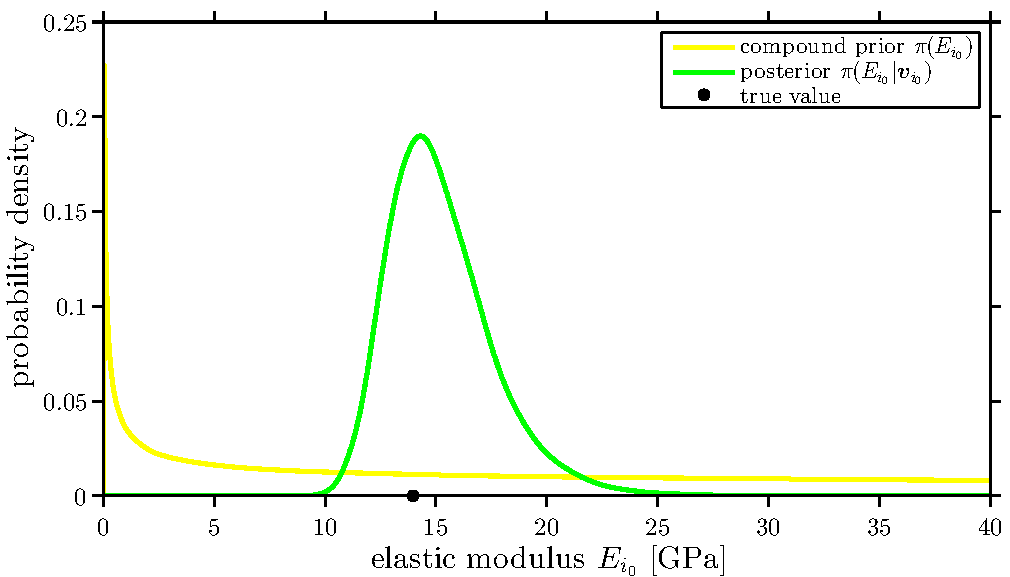
\includegraphics[height=\PEMfigHeight]{fig_PEM_CombInf1SimpleUpdating}
    \caption{Simple updating.}
    \label{fig:PEM:CombInf:SimpleUpdating}
  \end{subfigure}%
  \begin{subfigure}[b]{0.5\textwidth}
    \centering
    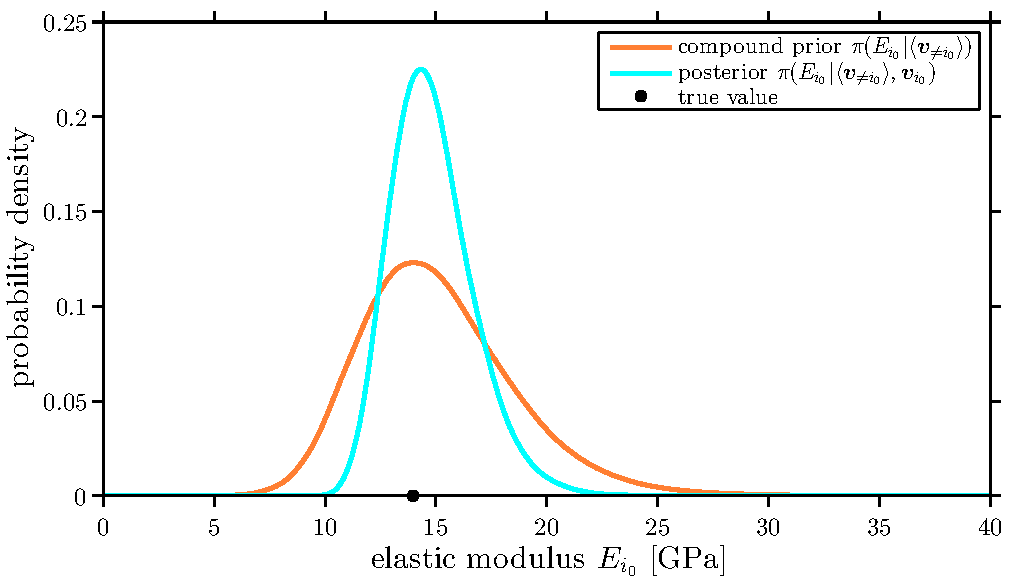
\includegraphics[height=\PEMfigHeight]{fig_PEM_CombInf1SequentialFiltering}
    \caption{Sequential filtering.}
    \label{fig:PEM:CombInf:SequentialFiltering}
  \end{subfigure}%
  \caption[Bayesian updating and filtering]{Bayesian updating and filtering.
           The mixture prior \(\pi(E_{\analyzed})\) and the posterior \(\pi(E_{\analyzed} \cond \bm{v}_{\analyzed})\) of simple updating are shown in \subref{fig:PEM:CombInf:SimpleUpdating}.
           Sequential filtering is based on the more informative mixture prior \(\pi(E_{\analyzed} \cond \tuple{\bm{v}_{\notanalyzed}})\) and the corresponding posterior
           \(\pi(E_{\analyzed} \cond \tuple{\bm{v}_{\notanalyzed}},\bm{v}_{\analyzed})\) that are given in \subref{fig:PEM:CombInf:SequentialFiltering}.
          }
  \label{fig:PEM:CombInf:UpdatingAndFiltering}
\end{figure}
%%%%%%%%%%%%%%%%%%%%%%%%%%%%%%%%%%%%%%%%%%%%%%%%%%%%%%%%%%%%%%%%%%%%%%%%%%%%%%%%%%%%%%%%%%%%%%%%%%%%%%%%%%%%%%%%%%%%%%%%%%%%%%%%%%%%%%%%%%%%%%%%%%%%%%%%%%%%%%%%%%%%%%%%%%%%%%%%%%%%%%%%%
\par % MULTILEVEL ANALYSIS
Lastly we perform Bayesian multilevel analysis as described in \cref{sec:PEM:CombInf:MultilevelAnalysis}.
% JOINT POSTERIOR
Sampling the joint posterior \(\pi(\tuple{E_i},\bm{\theta}_E \cond \tuple{\bm{v}_i})\) allows to straightforwardly extract samples
from its marginal \(\pi(E_{\analyzed} \cond \tuple{\bm{v}_{i}})\) in \cref{eq:PEM:CombInf:MultilevelAnalysis:Posterior}.
% MCMC
This is accomplished in \(t=\unit[4.57]{h}\) for \(N=10^7\) algorithm iterations.
% POSTERIORS SUMMARIES
The posterior and the previous inferential distributions relevant for \(E_{\analyzed}\) are plotted in \cref{fig:PEM:CombInf:Summary}.
In addition to that \cref{tab:PEM:CombInf:Summary} recapitulates the different approaches.
% SECOND SERIES OF RUNS
Results are also provided from a second series of runs that were independently carried out on top of the first one.
The motivation is to show that borrowing strength is a not a random but a systematic effect.
% ACCUMULATION OF INFORMATION
The accumulation of information concerning \(E_{\analyzed}\) manifests in the progressively decreasing uncertainty in the distributions.
At every stage of the estimation plan, a certain proportion of the available information has entered the analysis and has been translated into a gain of knowledge related to \(E_{\analyzed}\).
Only the multilevel posterior \(\pi(E_{\analyzed} \cond \tuple{\bm{v}_{i}})\) entirely aggregates the available information.
% FIGURES: SUMMARIES
\begin{figure}[ht]
  \centering
  \begin{subfigure}[b]{0.5\textwidth}
    \centering
    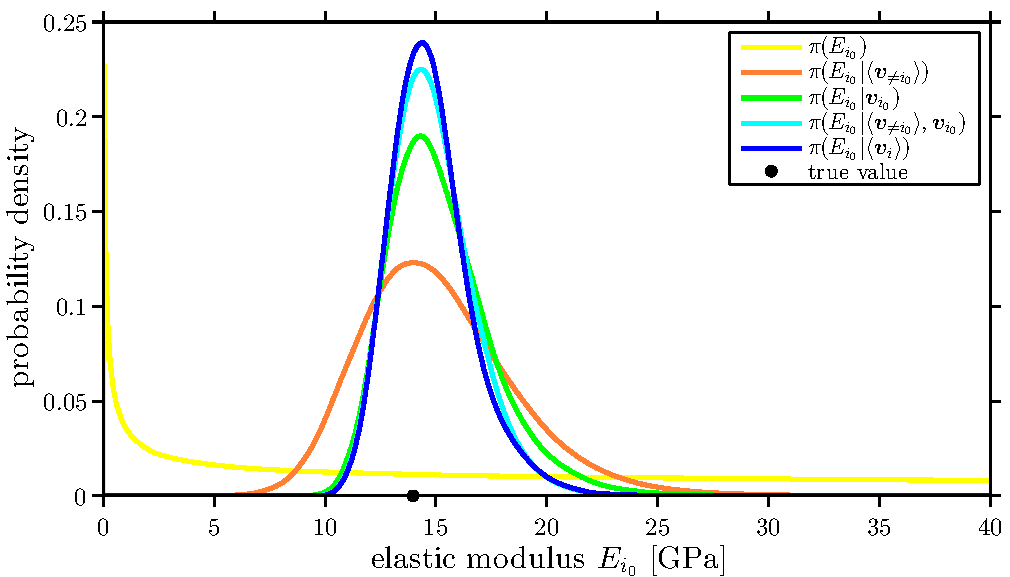
\includegraphics[height=\PEMfigHeight]{fig_PEM_CombInf1Summary}
    \caption{Summary of the \nth{1} series.}
    \label{fig:PEM:CombInf:Summary:1}
  \end{subfigure}%
  \begin{subfigure}[b]{0.5\textwidth}
    \centering
    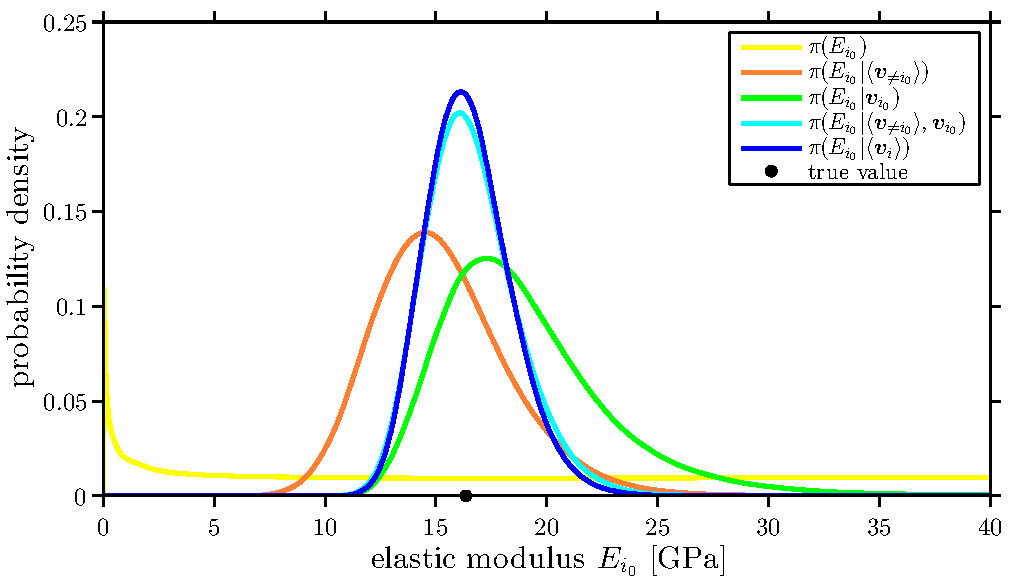
\includegraphics[height=\PEMfigHeight]{fig_PEM_CombInf2Summary}
    \caption{Summary of the \nth{2} series.}
    \label{fig:PEM:CombInf:Summary:2}
  \end{subfigure}%
  \caption[Accumulation of information]{Accumulation of information.
           In \subref{fig:PEM:CombInf:Summary:1} and \subref{fig:PEM:CombInf:Summary:2} the estimations of \(E_{\analyzed}\) are summarized for two series of runs.
           The true values are \(E_{\analyzed} = \unit[13.96]{GPa}\) and \(E_{\analyzed} = \unit[16.35]{GPa}\) in the \nth{1} and \nth{2} series, respectively.
           Uncertainties in identifying these values reflect the amount of information processed in simple updating, sequential filtering and multilevel inversion.
          }
  \label{fig:PEM:CombInf:Summary}
\end{figure}
% TABLE: OPTIMAL COMBINATION OF INFORMATION
\begin{table}[ht]
  \caption[Posterior summaries of estimating \(E_{\analyzed}\)]{Posterior summaries of estimating \(E_{\analyzed}\).}
  \label{tab:PEM:CombInf:Summary}
  \centering
  \begin{tabular}{lcccccccccc}
    \toprule
    & \phantom{} & \multicolumn{3}{c}{\nth{1} series: \(E_{\analyzed}\) \(\lbrack\unit[]{GPa}\rbrack\)} & \(\lbrack \unitless \rbrack\)
    & \phantom{} & \multicolumn{3}{c}{\nth{2} series: \(E_{\analyzed}\) \(\lbrack\unit[]{GPa}\rbrack\)} & \(\lbrack \unitless \rbrack\) \\
    \cmidrule{3-6} \cmidrule{8-11}
    && Mean & Mode & SD & CV && Mean & Mode & SD & CV \\
    \midrule
    Simple updating      && \(15.23\) & \(14.31\) & \(2.38\) & \(0.16\) && \(19.02\) & \(17.30\) & \(3.93\) & \(0.21\) \\
    Sequential filtering && \(14.82\) & \(14.32\) & \(1.83\) & \(0.12\) && \(16.58\) & \(16.07\) & \(2.03\) & \(0.12\) \\
    Multilevel inversion && \(14.75\) & \(14.37\) & \(1.79\) & \(0.12\) && \(16.47\) & \(16.12\) & \(1.85\) & \(0.11\) \\
    \bottomrule
  \end{tabular}
\end{table}
\par % UNCERTAIN LOADS
The assumption of well-known loads \(F_i\) may be overly optimistic in experimental practice.
As done in \cref{sec:PEM:CaseStudies:AddPres} one could attach an additional prescribed uncertainty to those model inputs.
In doing so we expect similar results accompanied by a weakening of borrowing strength.
% UNCERTAIN LOADS
Furthermore we expect an indirect form of borrowing strength also to occur for the inputs of a prescribed uncertainty type.
Actually the prescribed uncertainty model does not permit for learning about a specific \(F_{\analyzed}\) by borrowing strength directly from \(\tuple{\bm{v}_{\notanalyzed}}\).
However, by optimally estimating \(E_{\analyzed}\) also learning \(F_{\analyzed}\) would be indirectly strengthened.